\input preamble.tex
\begin{centering}
\Huge{\textbf{Prøve 01 i strømningsmåling}}\\
\end{centering}
\vskip 2cm 
Følgende kompetansemål er relevante for prøven:
\begin{itemize}[noitemsep]

	\item planlegge, utføre, vurdere kvalitet, sluttkontrollere og dokumentere arbeidet
	\item montere, konfigurere, kalibrere og idriftsettelse digitale og analoge målesystemer
\end{itemize}
\vskip 2.5pt 
Hjelpemidler:\begin{itemize}[noitemsep]
	\item Oppgave 1-8: Kalkulator og formelark
	\item Oppgave 9 Alle ikke kommuniserende
\end{itemize}

\vskip 5pt 
\vskip 10pt 
Alle ark som leveres inn skal ha elevens navn.
\vskip 2.5pt 
Oppgave 1-8 skal leveres på papir, etter levering kan eleven ta frem PC og svare på oppgave 9. 
\vskip 2.5pt 
Når oppgave 9 skal leveres kan elevene slå på trådløst nettverkt og sende oppgaven på mail til:
\vskip 2.5pt 
fred-olav.mosdal@skole.rogfk.no
\vskip 2.5pt 
I emnefeltet skal det stå: Flowprøve
\vskip 2.5pt
Oppgaven SKAL sendes fra skolemailen. 
\vskip 2cm   
Konaktinformasjon:
\begin{itemize}[noitemsep]
	\item Kontaktlærer: Fred-Olav Mosdal
	\item TLF: 90507684
\end{itemize}


\vfil \eject
%Slutt forside
Oppgave 1 (6p)%Navngi
\vskip 2.5pt 
a) Nevn 4 hastighetbaserte strømningsmålere. \\
\vskip 2.5pt 

\begin{tikzpicture}
	\draw[step=0.5cm,gray!20,very thin]  grid (17,4) ;
\end{tikzpicture}
\vskip 2.5pt 
b) Nevn 4 strømningsmålere som er basert på differansetrykk\\
\vskip 2.5pt 

\begin{tikzpicture}
	\draw[step=0.5cm,gray!20,very thin]  grid (17,4) ;
\end{tikzpicture}
\vskip 2.5pt 


Oppgave 2 (6p) %Definisjoner
\vskip 2.5pt 
a) Hva forteller Reynolds nummer oss? \\
\vskip 2.5pt 

\begin{tikzpicture}
	\draw[step=0.5cm,gray!20,very thin]  grid (17,11) ;
\end{tikzpicture}
\vskip 2.5pt 
\vfil\eject
b) Hva menes med massestrøm sett i forhold til volumstrøm? \\
\vskip 2.5pt 

\begin{tikzpicture}
	\draw[step=0.5cm,gray!20,very thin]  grid (17,6) ;
\end{tikzpicture}
\vskip 2.5pt 
\vskip 2.5pt 
\vfil\eject
Oppgave 3 (6p)%Enkel utregninger.
\vskip 2.5pt 
a) Konverter en volumetrisk strømningsrate på 345 l/m kvikksølv ($\rho=13546 kg/m³$ om til en masse strøm oppgitt i kg/h
\vskip 2.5pt 

\begin{tikzpicture}
	\draw[step=0.5cm,gray!20,very thin]  grid (17,2) ;
\end{tikzpicture}
\vskip 0.5cm 
b) Vi har et rør som det strømmer olje med en strømningsrate på 200 m³/h og en temperatur på 50°C. Begge seksjonene er etter schedule 40.  Den første delen av røret har dimensjon DN200 (ID=202.74mm) og den andre delen har dimensjon DN65 (ID=62.68mm)
$$\includegraphics[width=15.5cm]{aFlow01x02.eps}$$
Regn ut hastigheten til fluidet i hver av seksjonene. 
\vskip 2.5pt 

\begin{tikzpicture}
	\draw[step=0.5cm,gray!20,very thin]  grid (17,12) ;
\end{tikzpicture}
\vskip 2.5pt 
\vskip 2.5pt 
Oppgave 4 (6p) %Tegneoppgaver(blokkskjema skisse osv. 
\vskip 2.5pt 
a) Tegn en laminær strømningsprofil \\
\vskip 5cm
b) Tegn en turbulent strømningsprofil \\
\vskip 5cm 
% Her kommer oppgaver som skal kreve forklaringer eller forståelse
\vfil\eject
Oppgave 5 (6p) %Feilsøkings oppgave
\vskip 2.5pt
Hva vil være problemet om vi bruker en linær DP-celle i dette målesystemet? Du kan anta at systemet er kalibrert til å gi 20mA ved URV (øvre måleverdi). 
\vskip 2.5pt 
$$\includegraphics[width=10.5cm]{aFlow01x01.eps}$$
\\

\begin{tikzpicture}
	\draw[step=0.5cm,gray!20,very thin]  grid (17,11) ;
\end{tikzpicture}
\vskip 2.5pt 
\vfil \eject
Oppgave 6 (6p) % Tegn og forklar virkemåte
\vskip 2.5pt 
Tegn og forklar virkemåten til en coriolis strømningsmåler. 
\vfil \eject

Oppgave 7 (6p) % Tegn og forkalr virkemåte. 
\vskip 2.5pt 
Tegn og forklar virkemåten til en magnetiske strømningsmåler. 
\vfil \eject
Oppgave 8 (6p) % Regneoppgave
\vskip 2.5pt 
Vi har en vortex strømnigsmåler som måler måler drivstofforbruket til en  forbrenningsovn. Strømningsmåleren har en "k=2.33 liter per puls" Regn ut:
\vskip 1cm
a) frekvensen på pulsene med en strømningsrate på 5000 liter per time. 

\vskip 5pt 

\begin{tikzpicture}
	\draw[step=0.5cm,gray!20,very thin]  grid (17,3) ;
\end{tikzpicture}
\vskip 0.5cm

b) Forbukt brensel i liter etter at tellern har telt 1 000 000 pulser. 

\vskip 5pt 

\begin{tikzpicture}
	\draw[step=0.5cm,gray!20,very thin]  grid (17,3) ;
\end{tikzpicture}
\vskip 0.5cm

c) Tiden det vil ta for å få 500 000 pulser på telleren  ved en strømningsrate på 194167 liter i timen. 
\vskip 5pt 

\begin{tikzpicture}
	\draw[step=0.5cm,gray!20,very thin]  grid (17,12) ;
\end{tikzpicture}
\vskip 0.5cm
\vfil\eject
Tom side 
\vfil\eject
Oppgave 9 (12p) \\ %skal beskrive hvordan en jobb skal utføres. (Planlegg, besriv hvordan du ville gjenomført og dokumenter jobben)

\vskip 5pt 
RIV UT DENNE SIDEN FØR DU LEVERER
\vskip 5pt 
Du jobber i et firma som blant annet driver med produksjon av aceton. I forbindelse med destilasjonskollonen har det vært problemer med strømningmåleren på reflux linjen. Den er av type Rousemount Model 8800C Smart Vortex Flowmeter. \\
Temperaturen til acetonet i refluxlinjen er 100°C. Ved denne temperaturen har aceton en $\rho=693.7 kg/m³$ og en µ=0.17mPa s\\
$$\includegraphics[width=15.5cm]{i04060x01.eps}$$
Måleren tatt med inn til benksetting (bench commissioning, se side 2-2 i manual. Du skal utføre det som er beskrevet under "A configure". Jobben din er ferdig når du er kommet til B). Din leder ønsker at du setter URV så høyt som måleren kan måle med Aceton under de gitte betingelsene, og at du setter LRV så lavt som det er mulig. \\
\\
Rørlinjen som måleren står på er et DN25 Schedule 40 rør med ID=26.64mm\\\\
Beskriv hvordan du ville planlagt, gjennomført og dokumentert denne jobben.
\includepdf[page=-,angle=90]{../eq/afgvformler.pdf}
\end {document}
